En este capítulo se presenta a la empresa \textbf{Imagina S.A. de C.V.} exponiendo los diferentes procesos en los que se verá involucrado el sistema \textbf{SGIP}. En la segunda sección se definen las diferentes responsabilidades de cada uno de los actores\footnote{Stakeholders}.


\section{Empresa}

La empresa Recursos y Materiales Educativos Imagina S.A. de C.V.  que lleva más de diez años en el negocio de papelería, se dedica a la distribución y venta de material didáctico así como artículos de oficina,  de entre los cuales las ventas de cuadernos, lápices, plumas y colores generan la mayor cantidad de ingresos y cuenta con diez sucursales a lo largo de la República Mexicana.\\

El director de la empresa al llevar a cabo un análisis financiero concluyó que las pérdidas son muy considerables en los últimos meses de operación y que estas comenzaron desde el año 2016. Gran parte de estos resultados se debe a que el mecanismo que utiliza para llevar control de la mercancía que entra y sale de sus papelerías es por medio de una libreta para cada local y algunos formularios.\\

Por otro lado,  ha notado que las empresas que representan su competencia directa como \href{https://www.lumen.com.mx/}{Lumen} o \href{http://www.lareynademesones.com.mx/}{La reyna de mesones} tienen una mejora en ventas desde hace años debido a que proporcionan a sus clientes un catálogo en línea con el que pueden realizar pédidos desde su casa u oficina, o conocer qué productos venden para comparar los precios que más les convengan, así como sus sucursales y su  ubicación geográfica.\\

Por último, muchos de sus empleados no tienen actualmente registro de sus ventas realizadas, lo que le ha levantado las sospechas necesarias para optar por contratar a \textbf{Code Eaters} para la implementación de una solución de software.

En la figura \ref{fig:Organigrama} se encuentra un diagrama de bloques en el que se visualiza la estructura actual de la empresa.

\begin{figure}[hbtp!]
	\begin{center}	
		\fbox{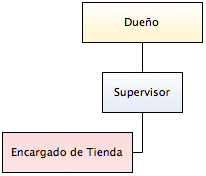
\includegraphics[width=0.5\textwidth]{contexto/img/Organigrama}}
		\label{fig:Organigrama}
		\caption{Organigrama de Imagina S.A. de C.V.}
	\end{center}
\end{figure}


\section{Stakeholders}

En la figura \ref{fig:Stake} se muestran a los actores que se definieron con ayuda del organigrama de la empresa.

\begin{figure}[hbtp!]
	\begin{center}	
		\fbox{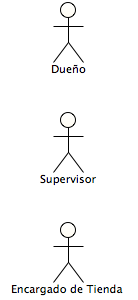
\includegraphics[width=0.1\textwidth]{contexto/img/Inventario_Actores}}
		\label{fig:Stake}
		\caption{Actores del Módulo de Inventario}
	\end{center}
\end{figure}


\begin{Stakeholder}{Dueño}
\item[Descripción]: Encargado de la empresa \textbf{Imagina S.A. de C.V.}.

        \item[Perfil:] Licenciatura
        \item[Responsabilidades:] \hspace{1em}
        \begin{itemize}
        	\item Proponer estrategias de mercadeo
		\item Establecer calendario de actividades
		\item Supervisar que las normas de la empresa se cumplan
		\item Autorizar o cancelar solicitudes de producto
		\item Entablar la comunicación con proveedores para llevar a cabo la compra de mercancia y asegurarse que se distribuya en aquellas tiendas que lo requieran
        \end{itemize}
        
\end{Stakeholder}

\begin{Stakeholder}{Supervisor}
		\item[Descripción:] Persona encarga de asegurarse que los Encargados de Tienda se encuentren laborando en sus respectivas tiendas.
		
        \item[Perfil:] Licenciatura en Administración industrial - logística
        
        \item[Responsabilidades:]\hspace{1em}
         \begin{itemize}
        	\item Dirigir al personal de cada tienda
		\item Levantar reportes de empleados
		\item Dar de alta nuevos productos	
        \end{itemize}
        
\end{Stakeholder}

\begin{Stakeholder}{Encargado de Tienda}
		\item[Descripción:] Persona encarga de vender productos así como de llevar un control del inventario.
		
        \item[Perfil:] Secundaria concluida.
        
        \item[Responsabilidades:]\hspace{1em}
         \begin{itemize}
        	\item Recibir productos
		\item Solicitar productos de acuerdo a su demanda o necesidad
		\item Abrir la tienda o cerrarla en el horario designado para ello
        \end{itemize}
\end{Stakeholder}



